\section{Implementation Details}

這次的作業要求我們實作多個 Key Components:

\begin{enumerate}
    \item \textbf{Multi-Head Attention 機制}:實作 Transformer 模型中的核心部分,使模型能夠理解圖像的上下文關係。
    
    \item \textbf{VQGAN 編碼理解}:深入了解 VQGAN 如何將圖片編碼成 256 個 token,每個 token 從 0-1023 範圍內選擇。這個過程類似於從 1024 個基本字母中,選用 256 個字母,並且有順序的組成一個句子來描述一張完整圖片。
    
    \item \textbf{Masked Visual Token Modeling}:實作訓練過程中的 forward 傳播和損失函數計算。
    
    \item \textbf{多階段生成過程}:實作圖像修補的生成流程,使模型能夠有效地填補圖像中的缺失部分。
\end{enumerate}



\subsection{The details of your model}

\paragraph{MultiHeadAttention} 在實作 Multi-Head Attention (MHA) 時,我們需要實作以下幾個步驟:

\begin{enumerate}
    \item 將輸入的圖像 token 進行線性變換,得到三個不同的向量:query、key 和 value。
    \item 將三個向量分別進行頭部劃分,得到多個頭部的向量。
    \item 計算每個頭部的注意力權重,並將其應用到對應的 value 向量上。
    \item 將多個頭部的向量進行拼接,得到最終的注意力權重。 
\end{enumerate}




\begin{lstlisting}[language=Python, caption=Multi-Head Attention 實作]
class MultiHeadAttention(nn.Module):
    def __init__(self, dim=768, num_heads=16, attn_drop=0.1):
        super(MultiHeadAttention, self).__init__()
        self.num_heads = num_heads
        self.dim = dim
        self.head_dim = dim // num_heads # 768//16 = 48
        self.qkv = nn.Linear(dim, dim * 3)
        self.proj = nn.Linear(dim, dim)
        self.attn_drop = nn.Dropout(attn_drop)
        self.scale = self.head_dim ** -0.5

    def forward(self, x):
        batch_size, num_image_tokens, dim = x.shape
        qkv = self.qkv(x)
        qkv = qkv.reshape(batch_size, num_image_tokens, 3, self.num_heads, self.head_dim)
        q, k, v = qkv.permute(2, 0, 3, 1, 4)
        attn = (q @ k.transpose(-2, -1)) * self.scale 
        attn = attn.softmax(dim=-1)
        attn = self.attn_drop(attn)
        x = (attn @ v).transpose(1, 2).reshape(batch_size, num_image_tokens, dim)
        x = self.proj(x)
        return x
\end{lstlisting}


我認為 MHA 成功的關鍵在於使用 Softmax 計算每個 Head 的注意力權重,這使模型能在生成圖像時考慮圖片中的多個重要區域。此外,根據 head\_dim 進行的縮放能有效地標準化模型的敏感度,使模型反應更加平滑而非過度尖銳,從而使訓練過程更加穩定和有效。


\subsection{The details of your stage2 training}

\paragraph{VQGAN to Vocab (Masked Generative Image Transformer)}
在訓練 Bi-directional 的 Transformer 模型時,首先是處理輸入的部分,這次要我實作使用 VQGAN 把圖片編碼成 256 個 token,所以我們需要在 MaskGIT 的 Class 一開始Load VQGAN 的模型參數,以及建立一個 encode to z 的函數,透過呼叫 VQGAN 的 encode 函數,把圖片編碼成 256 個 token,並且回傳 codebook\_mapping 和 codebook\_indices,但其實我們只會用到 codebook\_indices,並且在 Bi-directional 的 Transformer 模型中,重新這 1024 個字母 Embedding 到 768 維度的空間中。

\begin{lstlisting}[language=Python, caption=MaskGIT 訓練實作]
class MaskGIT(nn.Module):
    def __init__(self, configs):
        super(MaskGIT, self).__init__()
        self.vqgan = self.load_vqgan(configs['VQ_Configs'])
    ...
    @torch.no_grad()
    def encode_to_z(self, x):
        codebook_mapping, codebook_indices, _ = self.vqgan.encode(x)
        return codebook_mapping, codebook_indices.reshape(codebook_mapping.shape[0], -1)
\end{lstlisting}


\subsubsection{Learning rate strategy}



\begin{lstlisting}[language=Python, caption=學習率策略實作]
optimizer = torch.optim.AdamW(self.model.parameters(), lr=args.learning_rate)
scheduler = torch.optim.lr_scheduler.ChainedScheduler([
    torch.optim.lr_scheduler.LinearLR(optimizer, start_factor=0.1, end_factor=1.0, total_iters=args.warmup_epochs),
    torch.optim.lr_scheduler.CosineAnnealingLR(optimizer, T_max=args.epochs-args.warmup_epochs)
])
\end{lstlisting}

由於這次訓練的時間長度非常長,所以我沒有太多時間可以嘗試不同的學習率策略與 Optimizer,所以這次我使用的是最基本的學習率策略,就是使用 LinearLR 來進行 warmup 和 CosineAnnealingLR 來進行學習率策略以及 AdamW 的 Optimizer。 這是參考 LLama3 的訓練策略,並且也參考他們使用的 Learning rate 數值,設定成 8.0e-5。


\subsubsection{Dynamic Masking Ratio when training}




\begin{lstlisting}[language=Python, caption=動態遮罩比例實作]
mask = torch.bernoulli(torch.rand(z_indices.shape, device=z_indices.device) * 0.75 + 0.25).bool()
new_indices = mask * mask_token + (~mask) * z_indices
\end{lstlisting}


由於生成的時候,模型可能會面對到不同長度的 mask image,所以這裡我使用 25\% 到 100\% 的隨機比例生成 mask,可以模擬不同程度的訊息彌補任務。



\subsection{The details of your inference for inpainting task }

\paragraph{using Masked Generative Image Transformer}
\subsubsection{Gamma strategy}


由於生成的時候,雖然模型會把所有的 token 的 vocab 都生成出來,但是 transformer 同時生成多個 token 會有一個問題,會缺乏統一性,所以我們需要一個策略來多次生成 token,模型會先生成所有的 token,接著由於我們有每個 token 對應到每個字母的機率,所以我們可以保留機率高的,也就是我們認為模型生成的 token 是比較好的,接著我們會把機率低的 token 拔掉,這樣我們就可以得到一個比較好的生成結果。


這裏助教要求三種 gamma 函數,分別是 linear, cosine, square,這裏我突發起想,想說如果先大膽生成 token,然後再花一些步驟拔除那些多數 token 生成之後,信心度變低的 token,並且重新生成,會不會比較好的圖像品質呢?所以我設計了 sine\_linear。

我們使用以下的數學式來設計 sine linear gamma 函數:

\begin{equation}
    \gamma(r) = (1-r)(1-0.75\sin(2\pi r))
\end{equation}

其中 $r$ 是目前生成的比例 (0 到 1 之間)。這個函數有以下特性:

\begin{itemize}
    \item 當 $r=0$ 時, $\gamma(0)=1$, 代表一開始要生成所有 token
    \item 當 $r=1$ 時, $\gamma(1)=0$, 代表最後所有 token 都要確定
    \item $\sin(2\pi r)$ 項讓函數在生成過程中有大膽生成 token 的階段以及,移除信心不高的 token 的階段。
    \item 0.75 係數控制波動的幅度
    \item $(1-r)$ 項確保整體遞減趨勢
\end{itemize}



\begin{lstlisting}[language=Python, caption=Gamma 函數實作]
def gamma_func(self, mode="linear"): 
    gamma_funcs = {
        "linear": lambda r: 1 - r,
        "cosine": lambda r: np.cos(r * np.pi / 2),
        "square": lambda r: 1 - r ** 2,
        "sqrt": lambda r: 1 - np.sqrt(r),
        "sine_linear": lambda r: (1 - r) * (1 - np.sin(2 * np.pi * r)  *  0.75),
        "constant": lambda r: np.zeros_like(r)
    }
    if mode not in gamma_funcs:
        raise NotImplementedError
    return gamma_funcs[mode]
\end{lstlisting}


\begin{figure}[h]
    \centering
    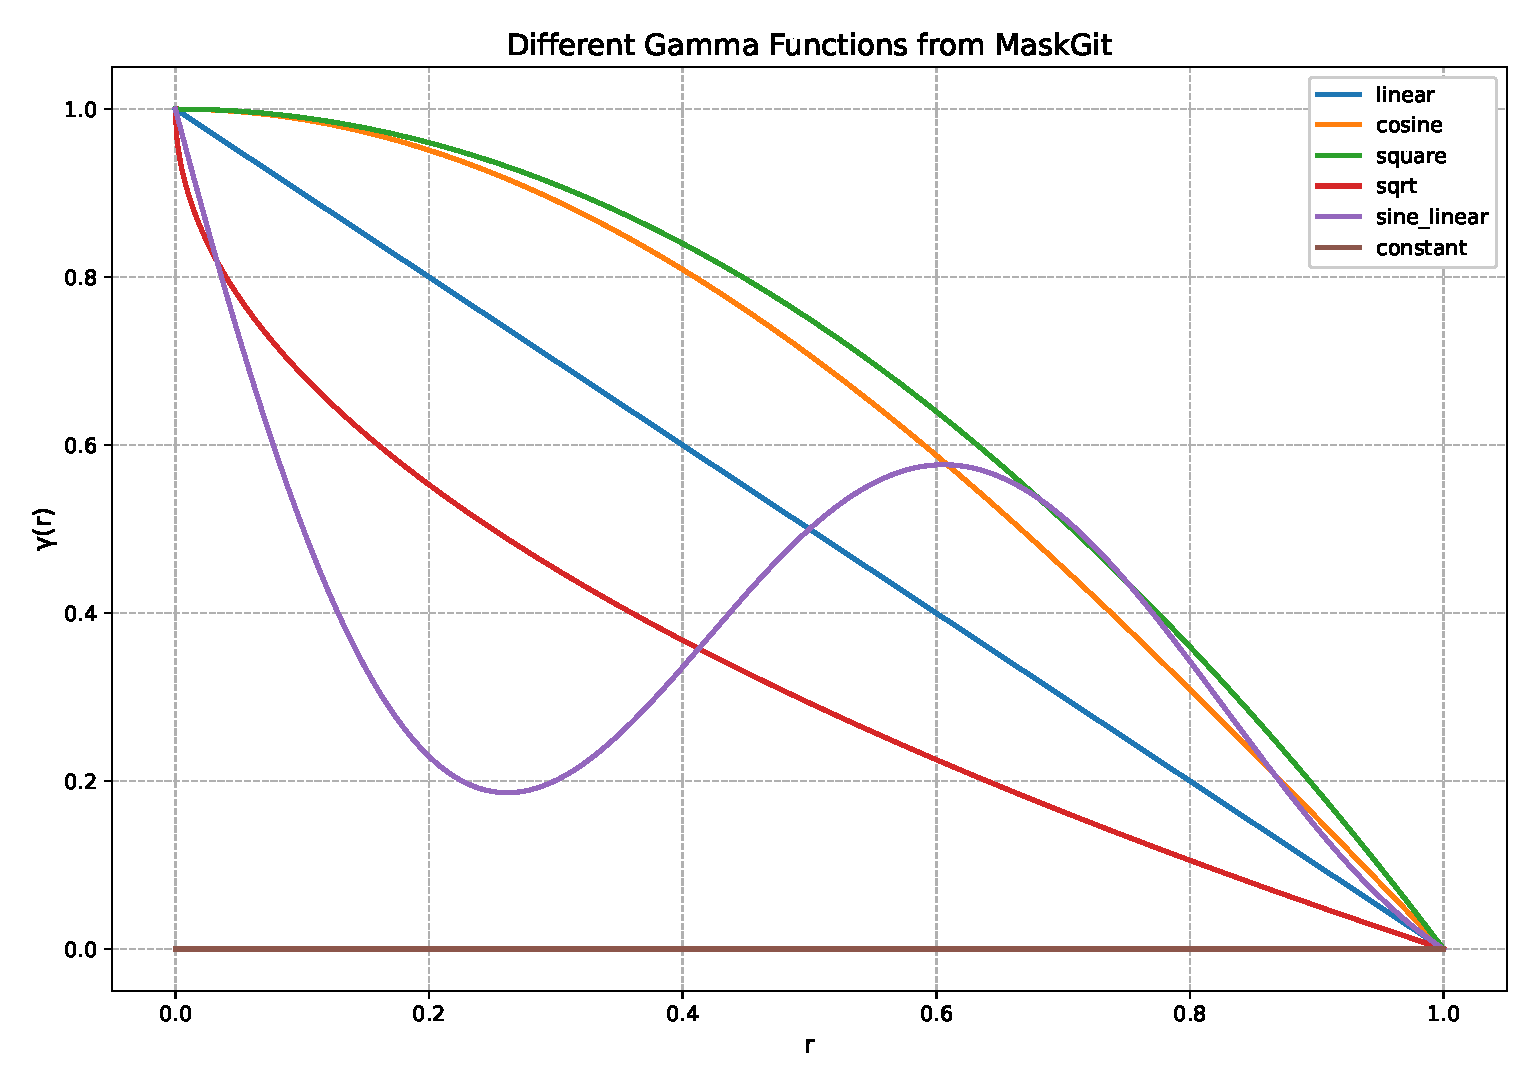
\includegraphics[width=\textwidth]{figures/gamma_functions}
    \caption{不同的 gamma 函數策略}
    \label{fig:gamma_functions}
\end{figure}


\subsubsection{Inpainting Implementation}

在修補圖片的過程中,首先我們要先取得 token,但由於我們每個區域的大小是 4x4 ,所以如果有部分區域被 mask 掉,我們需要直接把全部的 token 都填入 Mask token 這個特殊的 token。

然後再使用我們訓練出來的雙向 transformer 來進行 sequence 到 sequence 的轉換任務,然後由於我們的 batch size 是 1 來生成圖片,所以我們要用 logits 去除 batch 的維度,接著 transforemr 就預測我們每個位置的 token 機率,此時要把特殊的 mask token 設定是機率為 0,然後這邊由於是生成任務,所以我們讓模型是基於機率去抽樣,而不是總是選擇機率最高的token,接著我們把不在 mask 中的 token 設定是機率非常高,代表我們不用移除這些確定的 token,然後在 sorting 的時候,透過加入隨機數值到到 token 的機率矩陣中,讓排序也有隨機性,並且當 step 進行到越後面的時候,讓這個隨機性減小。

\begin{lstlisting}[language=Python, caption=Inpainting 函數實作]
@torch.no_grad()
def inpainting(self, z_indices_predict, mask_bc, mask_num, step_ratio, mask_func):
    z_indices_with_mask = mask_bc * self.mask_token_id + (~mask_bc) * z_indices_predict
    logits = self.transformer(z_indices_with_mask)
    logits = logits[0]
    probs = F.softmax(logits, dim=-1)
    probs[:, self.mask_token_id] = 0
    probs = probs / probs.sum(dim=-1, keepdim=True)
    z_indices_predict = torch.multinomial(probs, num_samples=1).squeeze(-1)
    z_indices_predict_prob = probs.gather(1, z_indices_predict.unsqueeze(-1)).squeeze(-1)
    z_indices_predict_prob = torch.where(
        mask_bc,
        z_indices_predict_prob,
        torch.tensor(float('inf'), device=z_indices_predict_prob.device)
    )

    mask_ratio = self.gamma_func(mask_func)(step_ratio)
    mask_len = torch.floor(mask_num * mask_ratio).long()
    g = torch.distributions.gumbel.Gumbel(0, 1).sample(z_indices_predict_prob.shape).to(z_indices_predict_prob.device)
    temperature = self.choice_temperature * (1 - step_ratio)
    confidence = z_indices_predict_prob + temperature * g
    
    sorted_confidence = torch.sort(confidence, dim=-1)[0]
    cut_off = sorted_confidence[:, mask_len].unsqueeze(-1)
    new_mask = (confidence < cut_off)
    return z_indices_predict, new_mask
\end{lstlisting}


